\documentclass{article}
\usepackage{tikz} 
\usepackage{pgfplots} 
\usepackage{stix}
\usepackage{gillius}
\usepackage{ccicons}

\usepackage[margin=0in, includehead, includefoot, paperwidth=8.625in, paperheight=8.75in]{geometry}
\usetikzlibrary{backgrounds}
\usetikzlibrary{patterns}


\definecolor{scarlet}{RGB}{187,0,0}

\begin{document}
\pagenumbering{gobble}


\tikz[remember picture,overlay] \node[inner sep=0pt] at (current page.center){\includegraphics[height=8.75in]{starsBlue.jpg}};
%\tikz[remember picture,overlay] \node[inner sep=0pt] at (current page.center){\includegraphics[width=8.625in]{frontTemplate.png}};

\flushright

\begin{tikzpicture}[opacity=1]
  \node at (1,0) {\scalebox{4}{\Huge\textsf{\textbf{\textcolor{white}{calculus}}}}};
  \node at (8,1.19) {\scalebox{10}{\Huge\textsf{\textbf{\textcolor{white!65!black}{2}}}}};  %% Aligned with subtitle
  %\node at (8,1.85) {\scalebox{10}{\Huge\textsf{\textbf{\textcolor{white!65!black}{1}}}}}; %% Aligned with title
  \node at (1.1,-1.6) {\resizebox{4.8in}{.2in}{\Huge\textsf{\textcolor{white!65!black}
          {with free online interactive materials}
    }}};
    %\draw[yellow] (-9,-1.2)--(9,-1.2); %guide line
\end{tikzpicture}\hspace*{.3in}

\vspace{1in}


  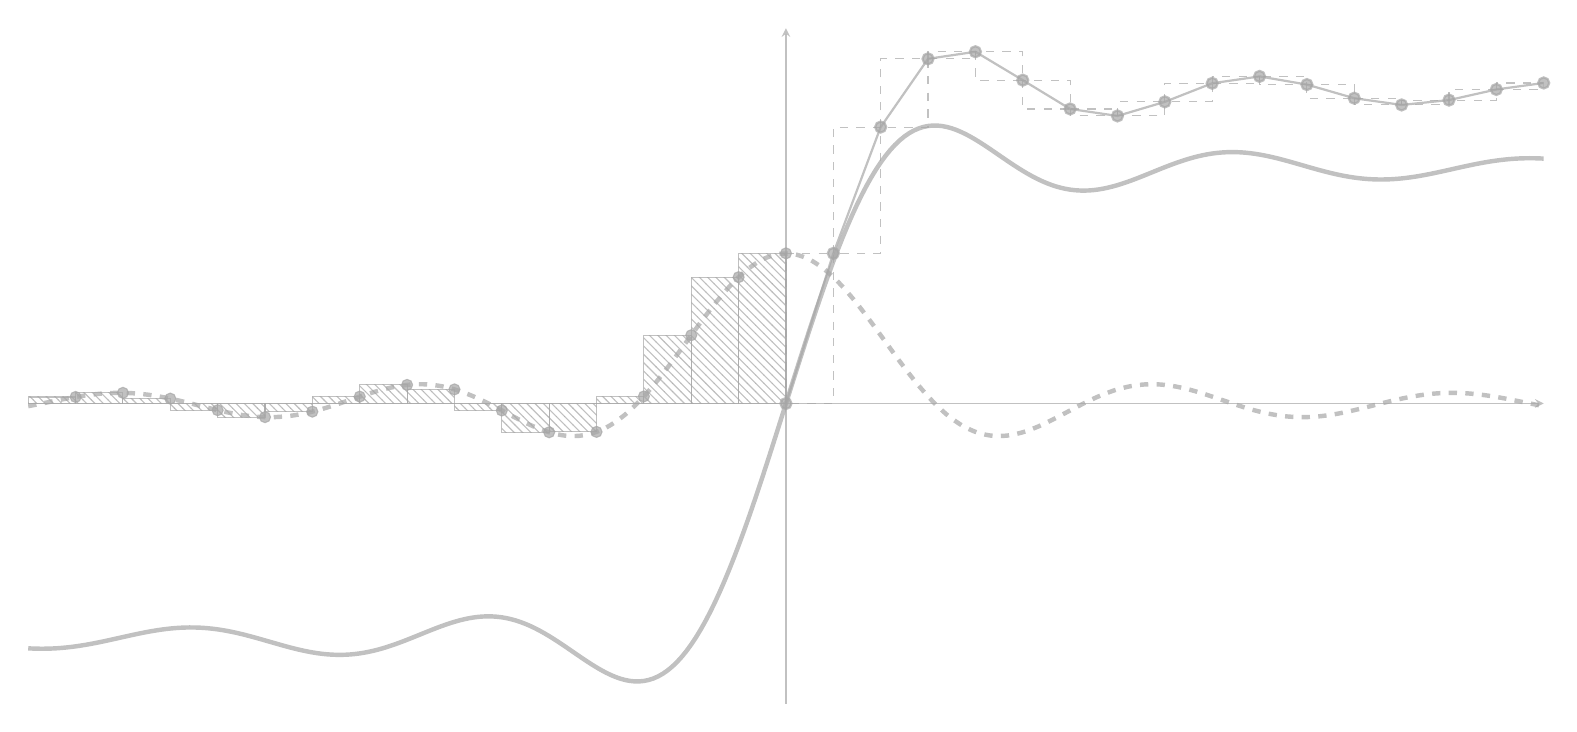
\begin{tikzpicture}[opacity =.7,declare function = {f(\x) = sin(deg(\x))/\x;}]]
    \begin{axis}[
        xmin=-16,
        xmax=16,
        ymin=-2,
        ymax=2.5,
        width=8.2in,
        height=4in,
        axis lines=middle, %xlabel=$x$, ylabel=$y$,
        every axis y label/.style={white!65!black,at=(current axis.above origin),anchor=south},
        every axis x label/.style={white!65!black,at=(current axis.right of origin),anchor=west},
        ticks=none,
        axis line style={white!65!black},
      ]
      \addplot [draw=white!65!black,pattern=north west lines, pattern color=white!65!black] plot coordinates %% last rect
               {({-1},{1})
                 ({0},{1})} \closedcycle;
      \foreach \rectnumber in {1,2,3,...,15} %% left hand rect
               {
                 \addplot [draw=white!65!black,%fill=gray!50!scarlet,
                   pattern=north west lines, pattern color=white!65!black] plot coordinates
                          {({(\rectnumber - 17)},{f(\rectnumber-16)})
                            ({1+(\rectnumber) -17 },{f(\rectnumber -16) })} \closedcycle;
               };


      %% Differential rectangles
      \draw[white!65!black,thin,dashed] (axis cs: 0, 0) rectangle (axis cs:1., 1.);
      \draw[white!65!black,thin,dashed] (axis cs: 1., 1.) rectangle (axis cs:2., 1.84147);
      \draw[white!65!black,thin,dashed] (axis cs: 2., 1.84147) rectangle (axis cs: 3., 2.29612);
      \draw[white!65!black,thin,dashed] (axis cs: 3., 2.29612) rectangle (axis cs: 4., 2.34316);
      \draw[white!65!black,thin,dashed] (axis cs: 4., 2.34316) rectangle (axis cs: 5.,2.15396);
      \draw[white!65!black,thin,dashed] (axis cs: 5., 2.15396) rectangle (axis cs: 6., 1.96217);
      \draw[white!65!black,thin,dashed] (axis cs: 6., 1.96217) rectangle (axis cs: 7., 1.9156);
      \draw[white!65!black,thin,dashed] (axis cs: 7., 1.9156) rectangle (axis cs: 8., 2.00946);
      \draw[white!65!black,thin,dashed] (axis cs: 8., 2.00946) rectangle (axis cs: 9.,2.13313);
      \draw[white!65!black,thin,dashed] (axis cs: 9.,2.13313) rectangle (axis cs: 10., 2.17892);
      \draw[white!65!black,thin,dashed] (axis cs: 10., 2.17892) rectangle (axis cs: 11., 2.12452);
      \draw[white!65!black,thin,dashed] (axis cs: 11., 2.12452) rectangle (axis cs:12., 2.03361);
      \draw[white!65!black,thin,dashed] (axis cs:12., 2.03361) rectangle (axis cs:13.,1.9889);
      \draw[white!65!black,thin,dashed] (axis cs:13.,1.9889) rectangle (axis cs: 14., 2.02122);
      \draw[white!65!black,thin,dashed] (axis cs: 14., 2.02122) rectangle (axis cs: 15., 2.09197);
      \draw[white!65!black,thin,dashed] (axis cs: 15., 2.09197) rectangle (axis cs: 16., 2.13533);


 %% right end points
      \addplot[white!65!black,only marks,mark=*] coordinates {
(-15., 0.0433525) (-14., 0.0707577)
(-13., 0.0323205) (-12., -0.0447144)
(-11., -0.0909082) (-10., -0.0544021)
(-9., 0.0457909) (-8., 0.12367) (-7.,0.0938552)
(-6., -0.0465692) (-5., -0.191785) (-4., -0.189201) 
(-3., 0.04704) (-2., 0.454649) (-1., 0.841471) (0., 1.)
      };
      
      %% Euler
      \addplot[white!65!black,thick,mark=*] coordinates {
(0, 0) (1., 1.) (2., 1.84147) (3., 2.29612) (4., 2.34316)
(5.,2.15396) (6., 1.96217) (7., 1.9156) (8., 2.00946)
(9.,2.13313) (10., 2.17892) (11., 2.12452) (12., 2.03361)
        (13.,1.9889) (14., 2.02122) (15., 2.09197) (16., 2.13533)
      };

      

      
      %% Sinc
      \addplot [ultra thick,dashed, white!65!black, smooth,samples=100,domain=-16:16] {f(x)}; %% sinc

      %% Sin Integral
      \addplot[white!65!black,ultra thick] coordinates {  %% sine integral
((-16., -1.6313) (-15.9, -1.6328) (-15.8, -1.6337) (-15.7, 
-1.63396) (-15.6, -1.63359) (-15.5, -1.63258) (-15.4, -1.63093) 
(-15.3, -1.62865) (-15.2, -1.62575) (-15.1, -1.62226) (-15., 
-1.61819) (-14.9, -1.6136) (-14.8, -1.60851) (-14.7, -1.60296) 
(-14.6, -1.59702) (-14.5, -1.59072) (-14.4, -1.58414) (-14.3, 
-1.57733) (-14.2, -1.57036) (-14.1, -1.5633) (-14., -1.55621) 
(-13.9, -1.54917) (-13.8, -1.54225) (-13.7, -1.53552) (-13.6, 
-1.52905) (-13.5, -1.52291) (-13.4, -1.51716) (-13.3, -1.51188) 
(-13.2, -1.50711) (-13.1, -1.50292) (-13., -1.49936) (-12.9, 
-1.49647) (-12.8, -1.4943) (-12.7, -1.49287) (-12.6, -1.49221) 
(-12.5, -1.49234) (-12.4, -1.49327) (-12.3, -1.49501) (-12.2, 
-1.49755) (-12.1, -1.50088) (-12., -1.50497) (-11.9, -1.50981) 
(-11.8, -1.51535) (-11.7, -1.52155) (-11.6, -1.52835) (-11.5, 
-1.53571) (-11.4, -1.54356) (-11.3, -1.55182) (-11.2, -1.56042) 
(-11.1, -1.56927) (-11., -1.57831) (-10.9, -1.58743) (-10.8, 
-1.59654) (-10.7, -1.60556) (-10.6, -1.61439) (-10.5, -1.62294) 
(-10.4, -1.63112) (-10.3, -1.63883) (-10.2, -1.646) (-10.1, 
-1.65253) (-10., -1.65835) (-9.9, -1.66338) (-9.8, -1.66757) 
(-9.7, -1.67084) (-9.6, -1.67316) (-9.5, -1.67446) (-9.4, 
-1.67473) (-9.3, -1.67393) (-9.2, -1.67205) (-9.1, -1.66908) 
(-9., -1.66504) (-8.9, -1.65993) (-8.8, -1.65379) (-8.7, 
-1.64665) (-8.6, -1.63857) (-8.5, -1.6296) (-8.4, -1.61981) 
(-8.3, -1.60928) (-8.2, -1.5981) (-8.1, -1.58637) (-8., -1.57419) 
(-7.9, -1.56167) (-7.8, -1.54894) (-7.7, -1.53611) (-7.6, 
-1.52331) (-7.5, -1.51068) (-7.4, -1.49834) (-7.3, -1.48644) 
(-7.2, -1.47509) (-7.1, -1.46443) (-7., -1.4546) (-6.9, -1.4457) 
(-6.8, -1.43787) (-6.7, -1.43121) (-6.6, -1.42582) (-6.5, 
-1.42179) (-6.4, -1.41922) (-6.3, -1.41817) (-6.2, -1.41871) 
(-6.1, -1.42087) (-6., -1.42469) (-5.9, -1.43018) (-5.8, 
-1.43736) (-5.7, -1.4462) (-5.6, -1.45667) (-5.5, -1.46872) 
(-5.4, -1.4823) (-5.3, -1.49732) (-5.2, -1.51367) (-5.1, 
-1.53125) (-5., -1.54993) (-4.9, -1.56956) (-4.8, -1.58998) 
(-4.7, -1.61101) (-4.6, -1.63246) (-4.5, -1.65414) (-4.4, 
-1.67583) (-4.3, -1.69732) (-4.2, -1.71837) (-4.1, -1.73874) 
(-4., -1.7582) (-3.9, -1.7765) (-3.8, -1.79339) (-3.7, -1.80862) 
(-3.6, -1.82195) (-3.5, -1.83313) (-3.4, -1.84191) (-3.3, 
-1.84808) (-3.2, -1.8514) (-3.1, -1.85166) (-3., -1.84865) (-2.9, 
-1.84219) (-2.8, -1.8321) (-2.7, -1.81821) (-2.6, -1.80039) 
(-2.5, -1.77852) (-2.4, -1.75249) (-2.3, -1.72221) (-2.2, 
-1.68762) (-2.1, -1.6487) (-2., -1.60541) (-1.9, -1.55778) (-1.8, 
-1.50582) (-1.7, -1.44959) (-1.6, -1.38918) (-1.5, -1.32468) 
(-1.4, -1.25623) (-1.3, -1.18396) (-1.2, -1.10805) (-1.1, 
-1.02869) (-1., -0.946083) (-0.9, -0.860471) (-0.8, -0.772096) 
(-0.7, -0.681222) (-0.6, -0.588129) (-0.5, -0.493107) (-0.4, 
-0.396461) (-0.3, -0.298504) (-0.2, -0.199556) (-0.1, -0.0999445) 
(0., 0.) (0.1, 0.0999445) (0.2, 0.199556) (0.3, 0.298504) (0.4, 
  0.396461) (0.5, 0.493107) (0.6, 0.588129) (0.7, 0.681222) (0.8, 
  0.772096) (0.9, 0.860471) (1., 0.946083) (1.1, 1.02869) (1.2, 
  1.10805) (1.3, 1.18396) (1.4, 1.25623) (1.5, 1.32468) (1.6, 
  1.38918) (1.7, 1.44959) (1.8, 1.50582) (1.9, 1.55778) (2., 
  1.60541) (2.1, 1.6487) (2.2, 1.68762) (2.3, 1.72221) (2.4, 
  1.75249) (2.5, 1.77852) (2.6, 1.80039) (2.7, 1.81821) (2.8, 
  1.8321) (2.9, 1.84219) (3., 1.84865) (3.1, 1.85166) (3.2, 
  1.8514) (3.3, 1.84808) (3.4, 1.84191) (3.5, 1.83313) (3.6, 
  1.82195) (3.7, 1.80862) (3.8, 1.79339) (3.9, 1.7765) (4., 
  1.7582) (4.1, 1.73874) (4.2, 1.71837) (4.3, 1.69732) (4.4, 
  1.67583) (4.5, 1.65414) (4.6, 1.63246) (4.7, 1.61101) (4.8, 
  1.58998) (4.9, 1.56956) (5., 1.54993) (5.1, 1.53125) (5.2, 
  1.51367) (5.3, 1.49732) (5.4, 1.4823) (5.5, 1.46872) (5.6, 
  1.45667) (5.7, 1.4462) (5.8, 1.43736) (5.9, 1.43018) (6., 
  1.42469) (6.1, 1.42087) (6.2, 1.41871) (6.3, 1.41817) (6.4, 
  1.41922) (6.5, 1.42179) (6.6, 1.42582) (6.7, 1.43121) (6.8, 
  1.43787) (6.9, 1.4457) (7., 1.4546) (7.1, 1.46443) (7.2, 
  1.47509) (7.3, 1.48644) (7.4, 1.49834) (7.5, 1.51068) (7.6, 
  1.52331) (7.7, 1.53611) (7.8, 1.54894) (7.9, 1.56167) (8., 
  1.57419) (8.1, 1.58637) (8.2, 1.5981) (8.3, 1.60928) (8.4, 
  1.61981) (8.5, 1.6296) (8.6, 1.63857) (8.7, 1.64665) (8.8, 
  1.65379) (8.9, 1.65993) (9., 1.66504) (9.1, 1.66908) (9.2, 
  1.67205) (9.3, 1.67393) (9.4, 1.67473) (9.5, 1.67446) (9.6, 
  1.67316) (9.7, 1.67084) (9.8, 1.66757) (9.9, 1.66338) (10., 
  1.65835) (10.1, 1.65253) (10.2, 1.646) (10.3, 1.63883) (10.4, 
  1.63112) (10.5, 1.62294) (10.6, 1.61439) (10.7, 1.60556) (10.8, 
  1.59654) (10.9, 1.58743) (11., 1.57831) (11.1, 1.56927) (11.2, 
  1.56042) (11.3, 1.55182) (11.4, 1.54356) (11.5, 1.53571) (11.6, 
  1.52835) (11.7, 1.52155) (11.8, 1.51535) (11.9, 1.50981) (12., 
  1.50497) (12.1, 1.50088) (12.2, 1.49755) (12.3, 1.49501) (12.4, 
  1.49327) (12.5, 1.49234) (12.6, 1.49221) (12.7, 1.49287) (12.8, 
  1.4943) (12.9, 1.49647) (13., 1.49936) (13.1, 1.50292) (13.2, 
  1.50711) (13.3, 1.51188) (13.4, 1.51716) (13.5, 1.52291) (13.6, 
  1.52905) (13.7, 1.53552) (13.8, 1.54225) (13.9, 1.54917) (14., 
  1.55621) (14.1, 1.5633) (14.2, 1.57036) (14.3, 1.57733) (14.4, 
  1.58414) (14.5, 1.59072) (14.6, 1.59702) (14.7, 1.60296) (14.8, 
  1.60851) (14.9, 1.6136) (15., 1.61819) (15.1, 1.62226) (15.2, 
  1.62575) (15.3, 1.62865) (15.4, 1.63093) (15.5, 1.63258) (15.6, 
  1.63359) (15.7, 1.63396) (15.8, 1.6337) (15.9, 1.6328) (16., 
  1.6313)
      };
    \end{axis}
  \end{tikzpicture}\hspace*{.6in}

\vfill

\flushleft
\hspace*{.4in}\begin{tikzpicture}
  \node at (0,0) {\scalebox{1}{\Huge\textsf{\textcolor{white}{\ccbyncsa}}}};
  \node at (4,-.2) {\large\textsf{\textcolor{white}{developed in \textbf{XIMERA}}}};
\end{tikzpicture}
\vspace*{.2cm}

\end{document}


